\documentclass[../../dissertation.tex]{subfiles}
\begin{document}

Consider the example of a quantum walker on a discretely numbered cycle. It was
seen that the evolution operator associated with such a system is, as defined in equation \eqref{eq:coinedUnmarkedOperator}
\begin{equation}
	   U = S(C\otimes I), 
           \label{eq:coinedUnmarkedOperatorQiskit}
\end{equation}
%TODO: Decidir se menciono as equacoes do shift e da coin.
where $S$ is a shift operator, defined in equation \eqref{eq:coinedShiftOperator}
as 
\begin{equation}
          S = \ket{0}\bra{0} \otimes \sum_{x=-\infty}^{x=\infty} \ket{x+1}\bra{x} + \ket{1}\bra{1}\otimes \sum_{x=-\infty}^{x=\infty} \ket{x-1}\bra{x},
	  \label{eq:shiftMatrixQiskit}
\end{equation} 
that increments or decrements the position of the walker according to the coin operator $C$.\par
%TODO: Reescrever prox paragrafo.
Previously, this system was simulated in Python by coding its equations.  Now,
the focus is to study and implement a quantum circuit based on the work
presented by \cite{douglaswang07}. This approach relies on multi-controlled
CNOT gates in order to shift the state of the walker by $+1$ or $-1$, each with
a probability associated with the chosen coin, as can be seen in figure
\ref{fig:douglasWangShift}. 
\begin{figure}[!h]
  \centering
  \begin{subfigure}[t]{.4\textwidth}
    \centering
    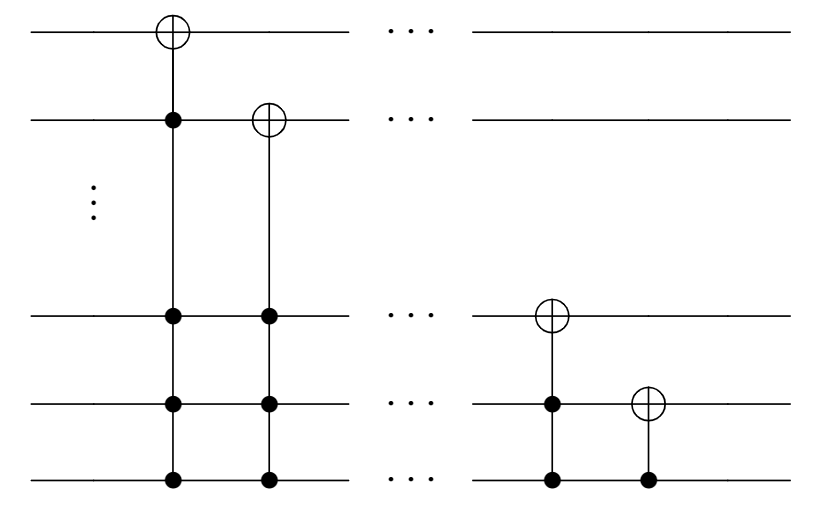
\includegraphics[width=\linewidth]{img/QCircuit/CoinedQuantumWalk/DouglasWangIncrement.png}
    \caption{Increment.}
  \end{subfigure}
  %\hfill
  \begin{subfigure}[t]{.4\textwidth}
    \centering
    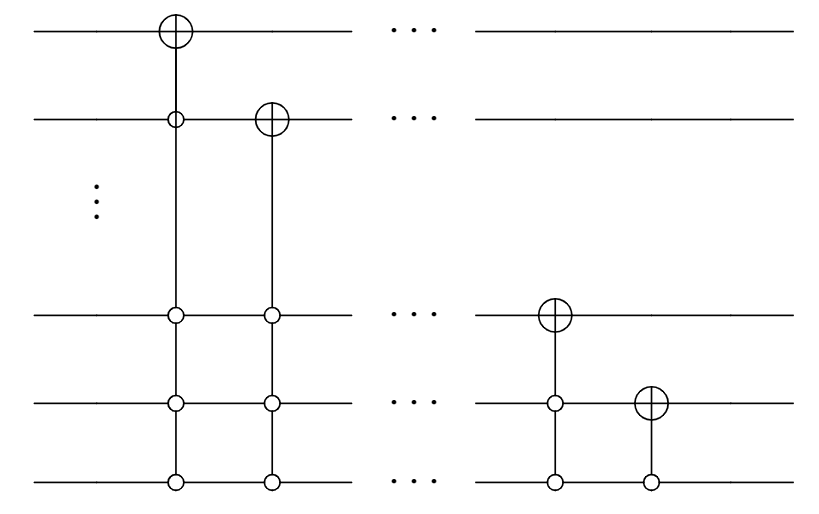
\includegraphics[width=\linewidth]{img/QCircuit/CoinedQuantumWalk/DouglasWangDecrement.png}
    \caption{Decrement.}
  \end{subfigure}
  \caption{General circuits of the components of the shift operator for the coined quantum walk.}
  \label{fig:douglasWangShift}
\end{figure}
%TODO: Melhorar o paragrafo seguinte
The generalized CNOT gates act on the vertex states as a cyclic permutator, where
each vertex state is mapped to an adjacent state. This can be seen as the walker moving
left or right, in the line graph example.
\begin{figure}[!h]
	\[ \Qcircuit @C=1.5em @R=1.3em {  & & &  \mbox{Repeat for steps.} & & &  \\ 
	               &  {/^{\otimes n}}\qw  &\qw           & \gate{\mbox{INCR}}     &  \gate{\mbox{DECR}}    & \qw \\
				   & \qw                             & \gate{\mbox{C}}                & \ctrlo{-1}           & \ctrl{-1}                   & \qw \gategroup{2}{3}{3}{5}{.8em}{--}      
		          } \]
	\centering
	\caption{General circuit for the coined quantum walk.}
	\label{fig:coinedCircuit}
\end{figure}\par
The coin operator will simply be a Hadamard gate acting on a single qubit. For
a graph of size $N=8$, for example, $n=3$ qubits are required to encode each
vertex, and an extra qubit for the coin. \par 

The general circuit for the
coined quantum walk is shown in figure \ref{fig:coinedCircuit}.
Note that this circuit limits the number of graph nodes to powers of $2$, and
an arbitrary implementation of $2^n$ nodes requires $n+1$ qubits.  However, it
is possible to have any number of nodes, given that the proper correction is
made, as was shown in the work of \cite{douglaswang07}. The method used for
this correction is called  \textit{Gray Code Ordering} proposed by
\cite{alexslepoy06}, whereby a certain arrangement of CNOT gates results in
control states only differing by a single bit.\par
\begin{figure}[!h]
	\centering
	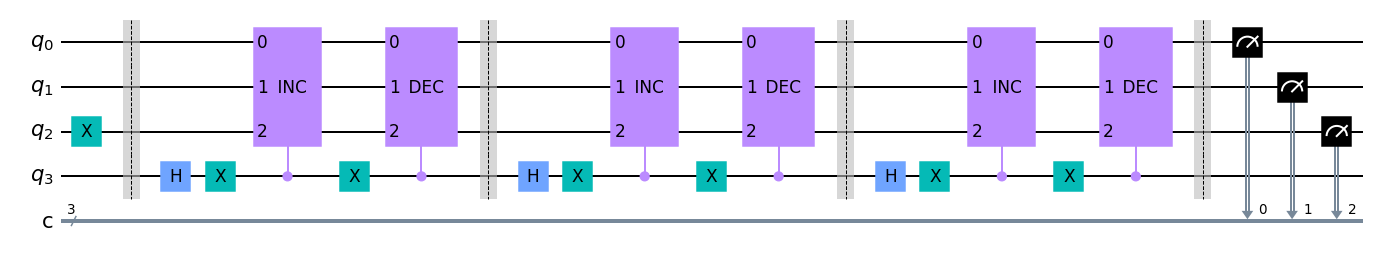
\includegraphics[scale=0.32]{img/Qiskit/CoinedQuantumWalk/Circuits/circCoinedQW_N3_S3.png}
	\caption{Qiskit circuit for the coined quantum walk, for a line graph of size $N=8$ and initial condition $\ket{\psi_0}=\ket{4}$, with 3 steps and the Hadamard coin.} 
	\label{fig:coinedQWCircuitQistkit}
\end{figure}
This circuit was implemented in Qiskit, as can be seen in figure
\ref{fig:coinedQWCircuitQistkit}. In this example, the increment and decrement
sequence was applied three times on a graph of size $2^3 =8$ nodes. The
starting position of the walker was set to $\psi(0) = \ket{4}$, and the
Hadamard coin was used. The first block after the barrier is the sequence of
operations that will increment the state of the walker, as shown in figure
\ref{fig:incrCircuitQistkit}. The generalized CNOT gates are implemented using
Qiskit's \textit{mcx} function, which implements the decomposition presented in
lemma 7.5 of \cite{barenco95} to create CNOT gates up to four controls, and the
aforementioned Gray Code for more generalized instances of the gate.
\begin{figure}[!h]
	\centering
	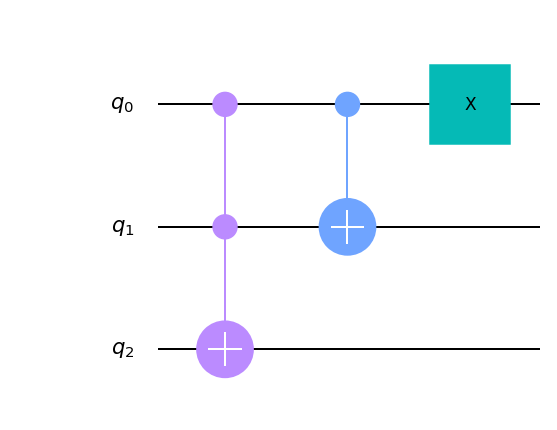
\includegraphics[scale=0.32]{img/Qiskit/CoinedQuantumWalk/Circuits/circIncr_N3_S3.png}
	\caption{Qiskit circuit of the increment operator for a line graph of size $N=8$.} 
	\label{fig:incrCircuitQistkit}
\end{figure}\par

The next set of operations perform the decrement of the state of the walker,
which is just an increment block with its controls negated, as is shown in
figure \ref{fig:decrCircuitQistkit}. The rest of the circuit is just the
repetition of these operations as a function of the number of steps required.
\begin{figure}[!h]
	\centering
	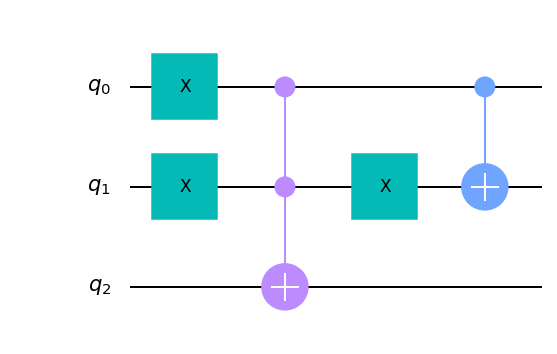
\includegraphics[scale=0.32]{img/Qiskit/CoinedQuantumWalk/Circuits/circDecr_N3_S3.png}
	\caption{Qiskit circuit of the decrement operator for a line graph of size $N=8$.} 
	\label{fig:decrCircuitQistkit}
\end{figure}\par

Lastly, the circuit is measured. The results can be seen in figure
\ref{fig:coinedQWQiskitDist}. These results can be verified by calculating the
time evolution of the wave function associated with the system
\begin{align}
	\ket{\psi(0)} &= \ket{4},\\
	\ket{\psi(1)} &= \frac{\ket{0}\ket{x=3}+\ket{1}\ket{x=5}}{\sqrt{2}}, \\
	\ket{\psi(2)} &= \frac{\ket{0}\ket{x=2}+\ket{1}\ket{x=4}+\ket{0}\ket{x=4}-\ket{1}\ket{x=6}}{2},\\
	\ket{\psi(3)} &= \frac{\ket{1}\ket{x=1}-\ket{0}\ket{x=3}+2(\ket{0}+\ket{1})\ket{x=5}+\ket{0}\ket{x=7}}{2\sqrt{2}}.
\end{align}
Taking the modulus squared of the amplitudes associated with the states,
confirms that the probability distribution associated with the \textit{QASM}
simulator, presented in figure \ref{fig:coinedQWQiskitDist} as the blue bar
plot, is correct. 
\begin{figure}[!h]
	\centering
	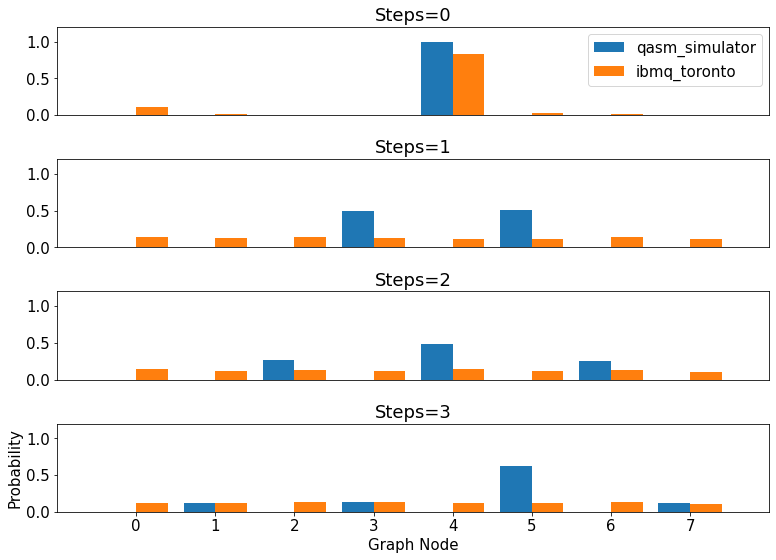
\includegraphics[scale=0.40]{img/Qiskit/CoinedQuantumWalk/CoinedQW_N3_S0123.png}
	\caption{Probability distributions of the coined quantum walk for several steps in a line graph of size $N=8$. The blue bar plot represents a circuit run in the QASM simulator, and the orange bar plot on IBM's Toronto backend.} 
	\label{fig:coinedQWQiskitDist}
\end{figure}
%TODO: Mencionar o numero de CNOTS?
However, the results obtained from running in IBM's \textit{Toronto} backend
are not satisfactory. This is because of the size of the circuit. Actually, the coined
quantum walk model besides requiring an extra qubit for the coin, also needs a
very large number of CNOT gates, which have an average associated error of
$1.284e^{-2}$ in this specific backend.\par

For a better error analysis, one can calculate the fidelity between the
ideal distribution $p(x)$ and the experimental $q(x)$ using the formula
\begin{equation}
    F(p,q) = \sum_{x=0}^{N-1} \sqrt{p(x)q(x)}
    \label{eq:bestFid}
\end{equation}
where $x$ is the vertex. For $0$ steps, the obtained fidelity is approximately
$0.91$ which is very high, because the circuit is simply the initial condition. When the circuit is increased to $1$ step the fidelity lowers to $0.49$,
due to the increase of CNOTs. However, for $2$ and $3$ steps, the fidelity
increases again to approximately $0.63$ due to the fact that the probability
distribution in the simulator becomes more spread out with the increase of
steps, meaning that the random uniform distribution obtained from the noisy
experiments ran in IBM's backend will be closer to them than a highly localized
distribution like in the case of $1$ step.\par

In order to reduce the effects introduced by noise, the next chapter will
present the circuit for the alternative discrete model, the staggered quantum
walk. Besides avoiding an extra qubit for the coin, this model also does not
require so many CNOT gates for each iteration.

\end{document}
